As monitors emit red, green, and blue light, this report will focus on these for LCA correction, however, it is worth noting that LCA applies to all wavelengths.

LCA causes blue light to be refracted further away from the normal than green and red due to its lower wavelength.
Similarly, red light is refracted less further away from the normal than green due to its higher wavelength.
As this happens radially, the further away from the centre of the lens, the greater the colour separation.
This occurs linearly in $r$, and is controlled by respective red, green, and blue coefficients.

Because of this, a pre-distortion correction for LCA is implemented in the fragment shader such that red light is magnified further than green light and green light is magnified further than blue light.
To show how this cancels out LCA, lens simulation is applied to the camera which includes both LCA and pincushion distortion.
LCA correction before and after lens distortion simulation are shown in Fig.~\ref{fig:lca-distortion} (a) and (b) respectively.

\begin{figure}[ht]
    \centering
    \subfloat[Correction]{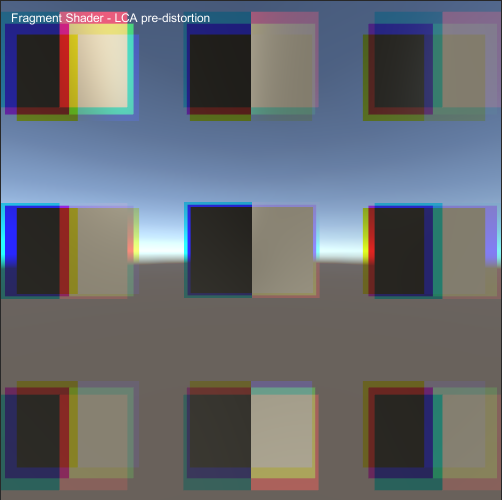
\includegraphics[width=0.35\textwidth]{figures/lca-correction}}
    \hfil
    \subfloat[Correction and Distortion]{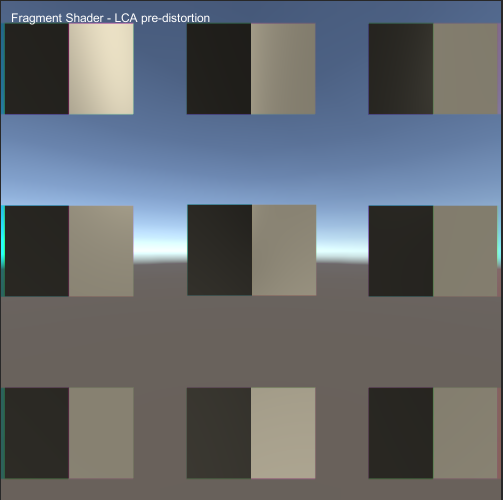
\includegraphics[width=0.35\textwidth]{figures/lca-distortion}}
    \caption{LCA pre-distortion and corrected LCA with distortion.}
    \label{fig:lca-distortion}
\end{figure}
